\documentclass{article}
\usepackage{amsmath,amsfonts,graphicx}



\begin{document}

\paragraph{4.1}

$U \cap V$ is open since,
\begin{eqnarray*}
U & = & X \slash \bar{U} \\
V & = & X \slash \bar{V} \\
U \cap V & = & X \slash \bar{U} \slash \bar{V}
\end{eqnarray*}
Therefore, remark 3.1.1 implies $f=g$ over $U \cup V$ is $U \cap V = 0$.  If $U \cap V$ is empty, then gluing $U$ and $V$ gives a regular function trivially.  That there exists a maximal $U$ on which $f$ is defined follows from homework exercise 1.7a(iv) with the above result.

\paragraph{4.2}
This result is symmetric to the above.

\paragraph{4.3}

\subparagraph{a} $f$ is defined when $x_0 \neq 0$ so the set is $P^2 \slash \{ x_0 = 0 \}$

\subparagraph{b} Begin by embedding $A^1_{y'}$ into $P^1$ via $y' \mapsto (y', 1)$.  So the induced map $\varphi : P^2 \to P^1$ is the mapping:
\[ \varphi(x_0, x_1, x_2) = (\frac{x_1}{x_0}, 1) \]
However, this map may be rationalized to give:
\[ \varphi(x_0, x_1, x_2) = (x_1, x_0) \]
Which is defined for all $P^2$.

\paragraph{4.4}

\subparagraph{a}
By exercise 3.1c, all conics in $P^2$ are isomorphic to $P^1$ and since isomorphism implies birational equivalence they are all rational curves.

\subparagraph{b}
Take the following projection:

\begin{center}
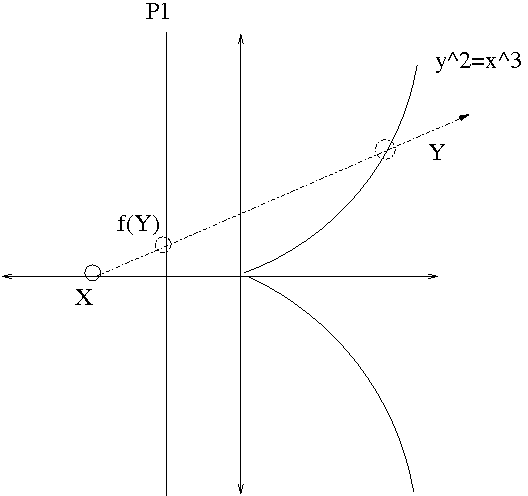
\includegraphics[width=3in]{birational.png}
\end{center}

Where the line $P^1$ is embedded as $x=0$ into $A^2$.  Fixing a point $X = (-1, 0)$ and taking the intersection of lines with $P^1$ gives a birational map between $P^1$ and the cuspidal cubic.  Therefore, the two sets are birationally equivalent.

\subparagraph{c}
This is identical to the above procedure.


\paragraph{5.1}

\begin{tabular}[h]{cccccc}
Problem & Picture & $f$ & $\partial_x f$ & $\partial_y f$ & Singular Points \\
a & Tacnode & $-x^2 + x^4 + y^4$ & $-2x + 4x^3$ & $4y^3$ & $(0,0)$ \\
b & Node & $x^6 - xy + y^6$ & $-2x + 4x^3$ & $4y^3$ & $(0,0)$ \\
c & Cusp & $-x^3 + x^4 + y^2 + y^4$ & $-3x^2 + 4x^3$ & $2y + 4y^3$ & $(0,0)$ \\
d & Triple Point & $x^4 - x^2 y  - xy^2 + y^4$ & $-3x^2 + 4x^3$ & $2y+4y^3$ & $(0,0)$ \\
\end{tabular}

\paragraph{5.2}

\begin{tabular}[h]{ccccccc}
Problem & Picture & $f$ & $\partial_x f$ & $\partial_y f$ & $\partial_z f$ & Singular Points \\
a & Pinch Point & $x y^2 - z^2$ & $y^2$ & $2xy$ & $-2z$ & $\{ y=0, z=0 \}$ \\
b & Conical Double Point & $x^2 + y^2 - z^2$ & $2x$ & $2y$ & $-2z$ & $\{ (0,0,0) \}$ \\
c & Double Line & $x^3 + xy +y^3$ & $3x^2 + y$ & $x+3y^2$ & $0$ & $\{ x=0, y=0 \}$ \\
\end{tabular}

\paragraph{5.6}

\subparagraph{a}
We handle both cases separately.  For the cusp we have the generators:

\begin{eqnarray*}
f_1 & = & -x^3 + x^4 + y^2 + y^4 \\
f_2 & = & x u - y t
\end{eqnarray*}

With the Jacobian matrix:
\[
\begin{pmatrix}
-3x^2 + 4x^3 & 2y+4y^3 & 0 & 0 \\
u & -t & x & -y
\end{pmatrix}
\]

Which is non-singular subject to $f_1=0, f_2=0$.

For the node, we get:

\begin{eqnarray*}
f_1 & = & x^6 - x y + y^6 \\
f_2 & = & x u - y t
\end{eqnarray*}

With the Jacobian matrix:
\[
\begin{pmatrix}
x^5 - y & y^5 - x & 0 & 0 \\
u & -t & x & -y
\end{pmatrix}
\]

\subparagraph{b}
If there are two distinct tangents to $P$, then there must be two distinct lines through the point at $P$.  Intersecting with the blow-up variety then gives two distinct intersections.  As a result the intersection curve is no longer singular.

\subparagraph{c}
The generators of the blow up of 5.1a are given as follows:

\begin{eqnarray*}
f_1 & = & x^4 + y^4 - x^2 \\
f_2 & = & x u - y t
\end{eqnarray*}

\begin{center}
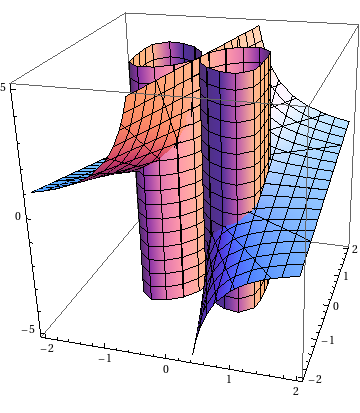
\includegraphics[width=3in]{blowup.png}
\end{center}

To compute the singular points; we now construct the Jacobian matrix of the generators of $\tilde{Y}$ for the two affine subspaces cut out by $t = 1$ and $u=1$:

For $t=1$:
\[
\begin{pmatrix}
-2x + 4x^3 & 4y^3 & 0 \\
u & -1 & x \\
\end{pmatrix}
\]

For $u = 1$:
\[
\begin{pmatrix}
-2x + 4x^3 & 4y^3 & 0 \\
1 & -t & y \\
\end{pmatrix}
\]

In both cases, the rank of the matrix is 2, since the bottom row vectors $(u,-1)$ and $(1,-t)$ do not contain any $x,y$ terms and the first row does not contain any constant or $u,t$ terms.  Since these two sets cover $A^2 \times P^1$, the local ring at all points in the variety is regular and thus $\tilde{Y}$ is nonsingular. 


\paragraph{7.1}

\subparagraph{a}

The $d$-uple embedding of $P^n$ in $P^N$ is given by the intersection of $n$ hypersurfaces of degree $d$.  Since this embedding is an isomorphism (exercise 3.4) and projective space is singly connected, there is exactly one intersection component in the image of the d-uple embedding with multiplicity 1.  Therefore, by theorem 7.7, the degree of the d-uple embedding is the product of the degree of each component and so it must be $d^n$. 

\subparagraph{b}
We showed that the Segre mapping was an isomorphism in problem 3.16.  Moreover, the Hilbert polynomial of $P^r$ is $\varphi_{P^r}(t) = { r + t \choose r }$ (using the argument on p.52) and so the Hilbert polynomial of the embedding, $Q$, is given by:
\begin{eqnarray*}
\varphi_{Q}(t)  & = & \varphi_{P^r}(t) \varphi_{P^s}(t) \\
& = & { r + t \choose r } { s + t \choose s } \\
\end{eqnarray*}
Looking at the leading coefficient for $\varphi_{Q}(t)$, we get $\frac{1}{r! s!} t^{r + s}$.  To solve for the degree of $Q$, $d$, we apply a second result from p.52 to see that:
\[ \frac{d}{(r + s)!} = \frac{1}{r! s!} \]
and thus 
\[ d = { r + s \choose r }  \]


\paragraph{7.5}

\subparagraph{a}

In dimension 1, for any point on the curve $Y$ there is some line (call it $H$) which intersects that point.  The intersection multiplicity of this line and that point is identical to the self-intersection multiplicity (by the definition from page 53).  So for each point that $H$ intersects $Y$ we have by theorem 7.7:
\[ \sum \limits_{x \in Y \cap H} i(Y, H ; x) = \textrm{deg } Y  \textrm{deg } H \]
However, $\textrm{deg } Y = d$ and $\textrm{deg } H = 1$ so the self intersection multiplicity for all points along $H$ is given by:
\[ \sum \limits_{x \in Y \cap H} i(Y, H ; x) = d \]
And therefore for any point the intersection multiplicity of that point must be strictly less than $d$.

\subparagraph{b}
Take a line tangent to that point, which then intersects the curve exactly once.  Because the line intersects the curve once, we may project the rest of $Y$ onto this tangent line using the method described in 4.4.


\paragraph{7.8}
The number of subspaces in $P^n$ is finite so there exists a minimum subspace containing $Y^r$ of dimensions $r+1$.

\end{document}
